\documentclass[a4paper,12pt,openany]{scrreprt}
\usepackage[
	left=2.5cm, 
	right=4cm, 
    top=2.5cm, 
    bottom=2.8cm,
    footskip=10mm,
    headsep=5mm]{geometry}

\usepackage[
	pdftitle={Linguistics Music Interface},
    pdfsubject={Module Paper - B.A. Linguistics - Bielefeld University},
    pdfauthor={Fabian Wohlgemuth},
    pdfkeywords={B.A., Module Paper, Bachelor, Linguistics, Music, Singing, Universität Bielefeld},
    %pdftex=true,
    colorlinks=true,
    citecolor=black,
    linkcolor=black,
    menucolor=black,
    urlcolor=black
]{hyperref}

\usepackage[utf8]{inputenc}
\usepackage[T1]{fontenc}
\usepackage{graphicx}
\usepackage{graphicx,subfigure}
\graphicspath{{images/}}
%\usepackage{fancyhdr}
\usepackage{lmodern}
\usepackage{color}
\usepackage[table,dvipsnames]{xcolor}
\usepackage{transparent}
\usepackage[ngerman,american]{babel}
\usepackage{lipsum}
\usepackage{datetime2}
\usepackage{setspace}
\onehalfspacing
\usepackage{tikz}
\usepackage{float}
\usepackage{amsmath}
\usepackage{amsfonts}
\usepackage{calc}
\usepackage{subfig}
\usepackage{csquotes}
\MakeOuterQuote{"} 

%%%
\input{pgfutil-common.tex}
\usepackage{pgfkeys,pgfmath}  
\usepackage{siunitx}

\newcommand{\printpercent}[3][2]{%  
    \pgfmathdivide{#2}{#3}% 
    \pgfmathmultiply{\pgfmathresult}{100}%
    \SI[round-mode=places,round-precision=#1]{\pgfmathresult}{\percent}
}
%%%

\usepackage[nottoc,notlot,notlof]{tocbibind}

\hypersetup{final}
\begin{document}

\pagestyle{empty}
\newgeometry{left=1.5cm,right=1.5cm,top=2cm,bottom=2cm}
\begin{center}

\Huge{\textbf{Universität Bielefeld}}

\LARGE{Fakultät für Linguistik und Literaturwissenschaft}

\vfill

\LARGE{\textbf{Hausarbeit}}

\Large

\href{https://ekvv.uni-bielefeld.de/sinfo/publ/modul/26797308}{23-LIN-BaLinS2}

\vfill

% On the Topic:

\vspace*{1cm}

\LARGE{\textbf{Unterschiede in der Phrasierung von gesprochenen und gesungenen Texten}\\\Large{am Beispiel zweier englischsprachiger Chor-Arrangements}}

\Large

\vfill

vorgelegt von

\vspace*{1cm}

\textbf{\href{https://fabianwohlgemuth.de}{Fabian Wohlgemuth}}

\vfill

$\begin{aligned}
\text{Begutachtet von:}&\ \text{Frau Prof. Dr. Petra Wagner}\\
% \text{Zweitgutachterin:}&\ \text{Frau Prof. Dr. Barbara Job}
\end{aligned}$

\vfill

\DTMlangsetup{showdayofmonth=false}
Bielefeld, \today
\DTMlangsetup{showdayofmonth=true}

\end{center}
\restoregeometry

\pagenumbering{Roman}

%\addcontentsline{toc}{section}{Danksagung}\setcounter{page}{2}\include{formalia/danksagung}
%\addcontentsline{toc}{section}{Abstract}\chapter*{Abstract}
\label{chap:Abstract}

% The following module paper looks at the current state of literature in the fields of language and music, to establish possible approaches to the interface between said fields.

%\addcontentsline{toc}{section}{Table of Contents}
\newpage
\tableofcontents

\newpage
\let\LaTeXStandardClearpage\clearpage
\let\clearpage\relax

%\begin{spacing}{1.1}
%\addcontentsline{toc}{section}{List of Figures/Tables}\listoffigures \listoftables
%\chapter*{Abkürzungsverzeichnis}
\label{chap:Abkürzungsverzeichnis}

\begin{acronym}[Bash]
% \acro{SMK}{Social Media Kommunikation}
\end{acronym}
%\end{spacing}

%\addtocontents{toc}{\vspace{\normalbaselineskip}}
%\addtocontents{toc}{\hrule}
%\addtocontents{toc}{\vspace{\normalbaselineskip}}
\let\clearpage\LaTeXStandardClearpage
\newpage
\pagenumbering{arabic}

\newpage
\chapter{Einleitung}
\label{chap:Einleitung}

\begin{quote}
\textit{''Music is the universal language of mankind.''}
\\--- Henry Wadsworth Longfellow

\textit{''Wer hört auf die Worte, wo Töne siegen!''} 
\\--- Richard Strauss, Capriccio (scene 3)
\end{quote}


\vspace{1cm}

% Zielsetzung - Problemstellung - Eingrenzung/Abgrenzung des Themas (begründet) - Aufbau - Roter Faden

\nocite{*}
\chapter{Literature Review}
\label{chap:Literature Review}
\pagestyle{plain}

\section{Phonetics and Phonology}
\label{Phonetics and Phonology}

Phoneticians study the minimal units that make up languages and the physical properties of their production and perception \cite{gudivada2018linguistics}. Phonology, other than phonetics, studies functionality of sounds, their behavior, and their organization \cite{davenport2013introducing}. 
Part of those studies of phonetics and phonology is prosody, where intonation and suprasegmentals are studied \cite{halliday1967intonation,fox2000prosodic}.

As \cite{nooteboom1997prosody} describes it, prosody, from the ancient Greek word for \textit{song sung with instrumental music}, is later being used for the science of versification and the laws of metre. Suprasegmentals like voice pitch, volume of speech, syllable lengths, and all their intentional modulations, are also part of prosody. The latter, including for example articulation (sharp vs. slurry), voice disguise by voluntary change of the larynx posture, or voicing (normal vs. hoarse vs. breathy), being essential to singing of given varieties of musical styles \cite{nooteboom1997prosody,thalen2001describing}.

The singing formant is a formant between F3 and F4, produced by male singers of western opera and concert singing \cite{sundberg1977acoustics}, explained by the typical larynx lowering in professional singing.

Crucial to phonetics and phonology, is the studying of the IPA chart, a chart of the International Phonetics Alphabet, by the International Phonetic Association. This chart contains sounds, diacritics, suprasegmentals, and tone and word accent symbols, to describe all possible sounds, a human can physically articulate. 

In singing, but especially in the choral singing context, knowledge of said chart can be an important advantage for singers and conductors \cite{adler1965phonetics}, for many choirs are singing pieces in multiple languages and thus, a larger range of phonemes are used. The differences in numbers of vowels --including the main singing languages of choral music-- can range between seven in Italian, to 16 in French.

The ability of pitch variation detection can be improved by singing abilities, as \cite{marques2007musicians} shows in a study, where French participants had to listen to sentences, spoken in Portuguese, where the pitch height on the final words were raised by 35 or 120 \% respectively. The results showed musicians being able to detect the 35 \% raise not only more often, but also being able to categorize congruous vs. incongruous endings 300 ms faster than the non musicians. This results are in line with an earlier study from \cite{schon2004music}.

One part, where linguistics intertwine with singing, is in vowels. As I can attest from different pieces sung by my choir, vowel identification is almost impossible above the mark of 700 Hz (concert tuning: F5) \cite{sundberg1977acoustics,sundberg2018phonetics}, often heard in high notes of avant-garde and opera pieces.

\cite{thalen2001describing} studied characteristics of this classical, and other singing styles. The results revealed that the female singer's voice source in Classical style was close to flow and neutral phonation. Pop and Jazz showed to be very close to the singer's neutral phonation. Only in Blues singing, there was a significant difference visible, as the singer's voice source was closest to her pressed phonation. In a later publication, Sundberg revisits the results of this publication and marks the topic as a still open research question, since the comparison of an artist's singing and speech behavior in more than the one aspect of the 2001 study, is very time consuming \cite{sundberg2003research}.

One interesting question arose in my planning for this module paper. What happens to the melody of song, sung in a tonal language. Or the other way round: What happens to the tones of the words in a tonal language, when sung as a text next to a melody. \cite{chan1987tone} researched tone and melody in Cantonese and found  modern songs in Mandarin to be melody dominant, so that the original tones of the lyrics seem to be ignored completely. In older Cantonese songs, melodies typically take lexical tones into consideration and attempt to preserve pitch contours and relative pitch heights, which either means, the words do not fit the melody, or, which is an overly complex task for the songwriter, the text is being written, so that the tones of the words fit the pitch changes in the melody.









\newpage
\section{Morphology and Syntax}
\label{Morphology and Syntax}

Morphology is the studying of words. How morphemes are built from the earlier learned phonemes and in what way morphemes can and cannot build new words in a given language. Syllable structure, with onset, nucleus, and coda, is defined by the morphology of a language. Also it describes rules of inflections, i.e. conjugation and declination \cite{bauer2003introducing}.

With built words, we can then form sentences, using syntactic rules of a given language. Syntax, from the Greek \textit{syntaxis}, meaning 'arrangement', studies the ways in which words are arranged to convey meaning within a sentence \cite{van2001introduction,matthews1982syntax}.

As for the syntax part, \cite{lerdahl1983overview} analyse J.S. Bach's chorale \textit{Ich bin's, ich sollte büssen} from the \textit{Matthäus-Passion BWV 244}, to establish \textit{a generative theory of tonal music} (GTTM) and to present hierarchical structure within music, as is already being used in linguistic analyses.
\cite{katz2011identity} are then extending on this 1983 model of musical structure, and say music to, like language, \textit{contain a syntactic component, building head structures by iterated, recursive, binary merge.} Also, the \textit{Time Span Reduction} by \cite{lerdahl1983overview} is argued to be a musical prosodic component, which strengthens the anticipations of music and language sharing structural elements.

\subsection*{Gaps in Findings}

When starting the literature review for this paper, I expected to find research on certain topics, that ended up being not as well researched as I expected. I want to point out those topics, that then will lead to an outlook with possible research topics for the future in \autoref{chap:Conclusion}.

Even though, stuttering is a subject, more researched in cognitive science, psycho- and neurolinguistics, I will add this paragraph to this section, as it influences the building of sentences. Stuttering, normally not occurring while singing, is a phenomenon, which is fairly well researched (e.g. in \cite{healey1976factors}). The reasons for it not occurring too much in singing, ranging from singing usually being with known text that does not allow surprises, which the brain needs to fill, to the fact, singing being not a way of communicating with one another, but is more of a monologue. Chris Martin, lead vocalist of \textit{Coldplay}, being a famous example for a stutterer. The research of \cite{healey1976factors}, being focused on cognitive changes between familiarity of melody and text, do not go into linguistically measurable differences and influences.








\section{Semantics and Pragmatics}
\label{Semantics and Pragmatics}

Semantics deal with the meaning of words and the meaning of words related to one another. The studies of pragmatics then deal with \textit{meaning variation with context} \cite{bagha2011short}.

In music, the meaning of the melody is an important factor, but at least as equally important as the meaning of the words, telling a story. \cite{zedda1998linguistic} quotes Christa Ludwig, interviewed by Gérard Mannoni: 

\blockquote{\textit{Chanter, ce n’est pas faire des sons, même très beaux. C’est d’abord savoir raconter une histoire.}

\textit{Singing is not about making sounds, even if they are beautiful. The most important thing is to be able to tell someone a story.}}

\cite{rossing2007springer}, too, speaks about the \textit{Expressive Power of the Human Voice} and about the meaning, that it can convey with subtle extra-linguistic variations of timing and pitch contour, timbre, and loudness. Those information are expressed in a way, that listeners can even replicate a speakers' facial expression by just listening to the voice, as shown in a study by \cite{fonagy1967horbare}.






\section{Language Learning and Multi-Lingualism}
\label{Language Learning and Multi-Lingualism}

One domain, in which music and language are often brought together, is language learning and multi-lingualism. Musical abilities are said to be a positive influence on language learning and vice versa.

The research of \cite{zeromskaite2014potential} finds ---though leading, by saying, that the little research done in this area, opposes a generalization of the results--- musically trained test subjects to have enhanced auditory and cognitive abilities, which \textit{contributes to the phonological and reading aspects of L2 acquisition}. 

In another study, \cite{ludke2014singing} got results, showing the singing domain to be superior to speaking, when learning foreign language phrases in an unknown language (here: Hungarian). In their study, a listen and repeat experiment was done in three domains: singing, rhythmic speaking, and speaking. The reproduction of the Hungarian phrases were significantly more accurate within the group of singing participants, so that they suggest the \textit{'listen and sing' learning method can facilitate verbatim memory for spoken foreign language phrases}.

\cite{roncaglia2016mastering} study this field the other way round and talk about the influence of multi-lingualism on musical perception. They say, that being multi-lingual with two languages with different rhythmic properties, enhances rhythm perception in music, \textit{providing further evidence of shared cognitive resources between language and music}. The study was done on Turkish learners of German and German learners of English. Another result of the study, that there was no difference between early and late learners, underlines the generality of this evidence.

The other way round, singing can also influence language abilities as well, as  \cite[abstract]{christiner2013song} describe it. They say, that singing performance is an indicator for speech imitation abilities. The retaining of certain plasticity and being open to new or unusual sound combinations are only two ways, professional singing helps to improve language abilities. They also found good singers to have improved memory span of auditory working memory.








\section{Other Branches}
\label{Other Branches}

To \textit{other branches}, I will for example count studies of psycho-linguistics, neurolinguistics, and computational linguistics, that will most certainly include research on the already established branches, but will either combine those, or even add other, tangential research topics and methods, to study human language. 

\subsection*{Gaps in Findings}

Next to the stuttering, I talked about in \autoref{Morphology and Syntax}, Accents in singing is another topic, I did not find too much research about. As stuttering, it may vary a lot between speaking and singing, and you might hear artists sing without being able to recognize accents that, in speaking, are fairly strong. Like with stuttering, this can occur through change of vocalization, that is normal while singing and often used as a way to blend the speaking voice into a specific style of music. The most easily recognizable variation being the lowered larynx and round vowels for the classical style in opposite to a raised larynx and sharper and brighter vowels in pop style music.

In computational linguistics, speech recognition is a main subject. The recognition process, in most cases, uses preferably a lot of speech data, to train a model, to be able to recognize phonemes, and with that, recognize words and phrases. But what, if the speech data is from singing recordings? \cite{mesaros2012singing} did a study on this, training their phoneme model on normal speech data, but then adopting it to certain voice characteristics, that differ from speaking to singing voice. Another way to train a phoneme model for speech recognition of sung words, could be the training on actual singing data instead of speech data. That, because of large differences in articulation while singing, needs comparably more data than the recognition via simpler speaking data. An interesting question, arising with this topic, is, whether the recognition of sung phrases increases or decreases the recognition accuracy in the process.

Another topic of computational linguistics is speech synthesis. Automatic announcements in the bus or the tram, or in some places in the internet, are fairly common these days. Combining speech synthesis with singing voice characteristics and melody, you could be able to synthesize singing. With the use of auto-tune, a software suite, that can improve singing, by tuning non-perfect sung notes to the closest correct note, computational linguistics and computational analysis of music are already a big part of the singing industry.
\chapter{Fazit und Ausblick}
\label{chap:Fazit und Ausblick}

% Ergebnisse zusammenfassen und bewerten - Beantworten der Fragen aus der Einleitung - Ausblick / Offene Fragen / Angrenzende Themengebiete
% KEINE neuen Erkenntnisse / Thesen



%% ---------------------------------------%%

%\pagestyle{plain}

\addtocontents{toc}{\vspace{\normalbaselineskip}}
\addtocontents{toc}{\hrule}
\addtocontents{toc}{\vspace{\normalbaselineskip}}

\pagenumbering{Roman}
\bibliographystyle{apalike}
\begin{doublespace}
\bibliography{mp_balins1.bib}
\end{doublespace}

\clearpage
\addcontentsline{toc}{chapter}{Declaration of Authorship}
\begin{doublespace}
\newgeometry{left=2.5cm,right=2.5cm,top=2cm,bottom=2cm}
%\doublespacing

{\let\clearpage\relax \chapter*{\centerline{Declaration of Authorship}}}
\label{chap:Declaration of Authorship}

\vspace*{1cm}

\setlength{\parindent}{0pt}
I hereby declare authorship of the module paper on hand. The module paper is entirely my own original work except where otherwise indicated. I am aware of the University's regulations concerning plagiarism, including those regulations concerning disciplinary actions that may result from plagiarism. Any use of the works of any other author, in any form, is properly acknowledged at their point of use.
\vspace*{2cm}

Bielefeld, \today \hfill \hrulefill

\hspace*{0mm}\phantom{Bielefeld, } 
\hfill Fabian Wohlgemuth\hspace*{1cm}
\restoregeometry
\end{doublespace}

%\addcontentsline{toc}{chapter}{Appendix}
%\chapter*{Anhang}
\label{chap:Anhang}

\begin{itemize}
  \item Run To You
  \item Fields Of Gold
\end{itemize}

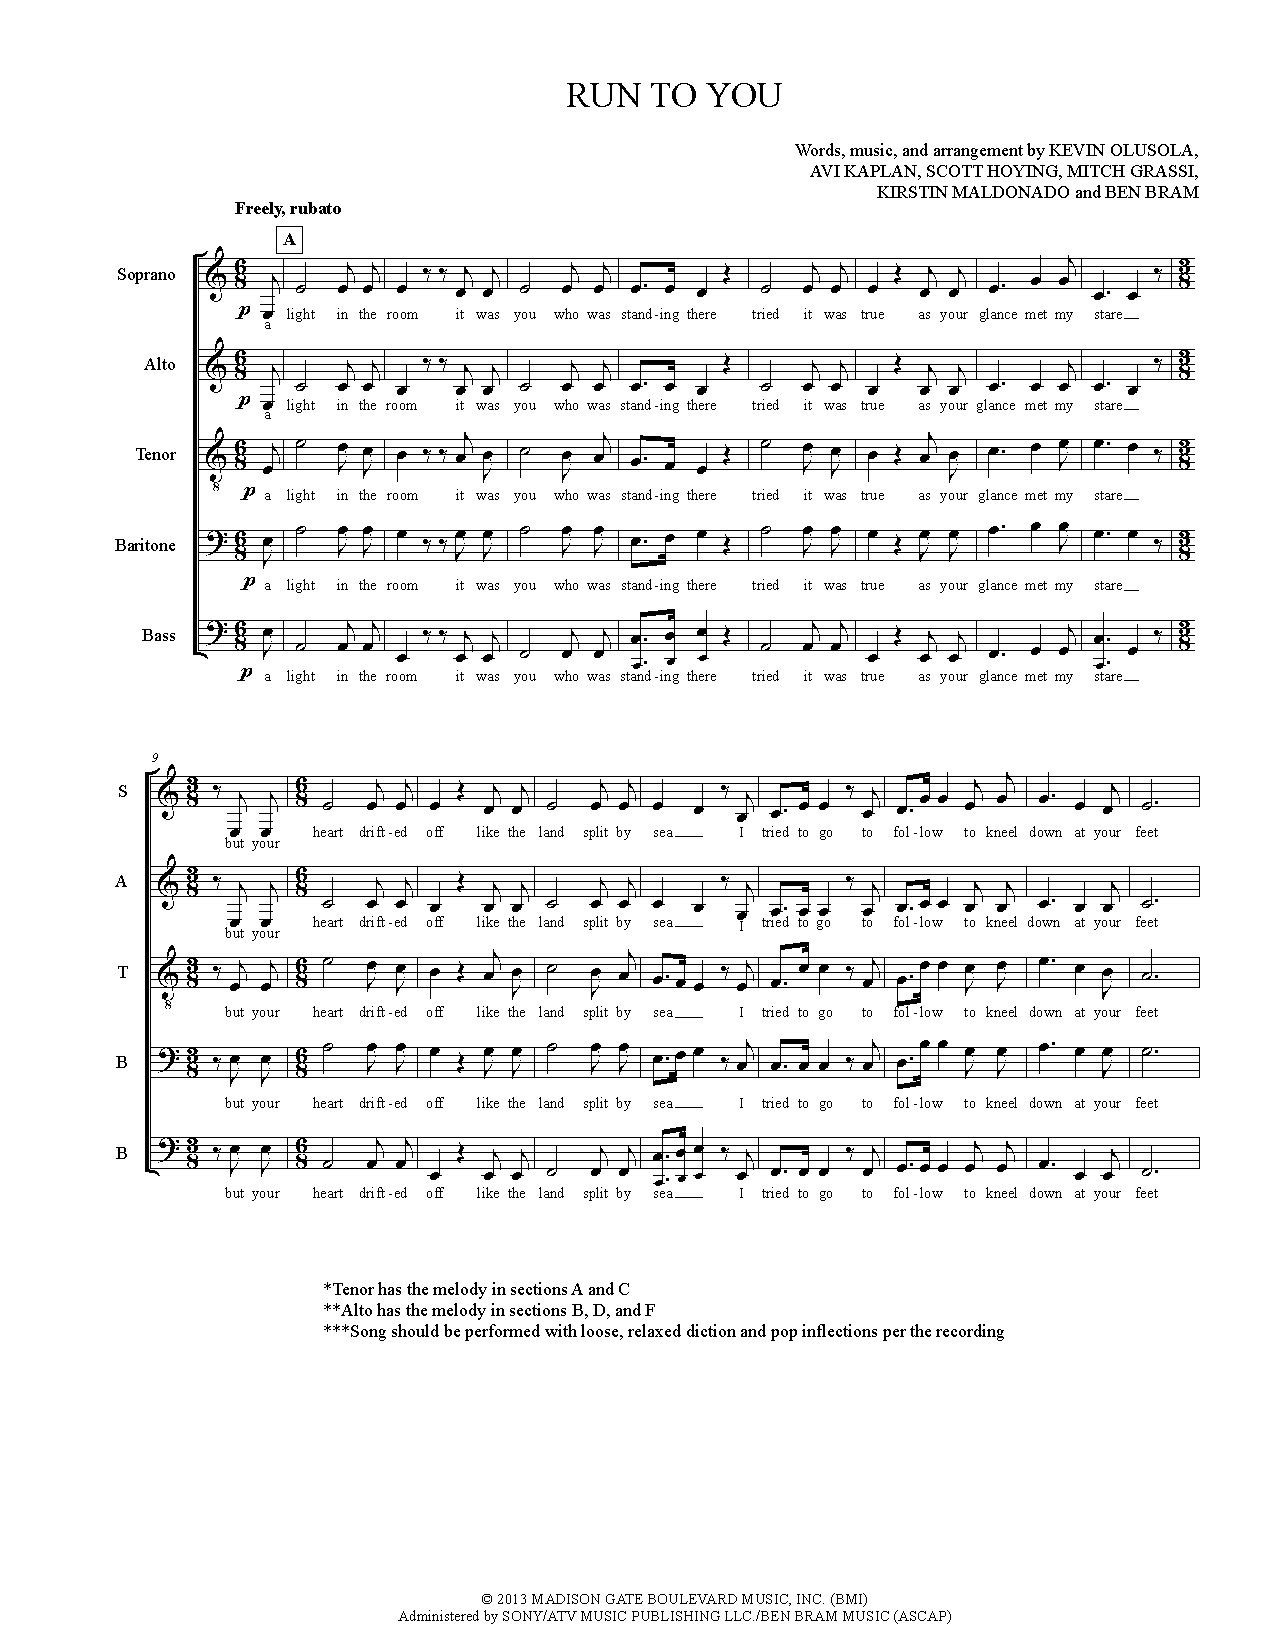
\includepdf[pages=-]{resources/arrangements/Run To You.pdf}
\label{appendix:Run To You}

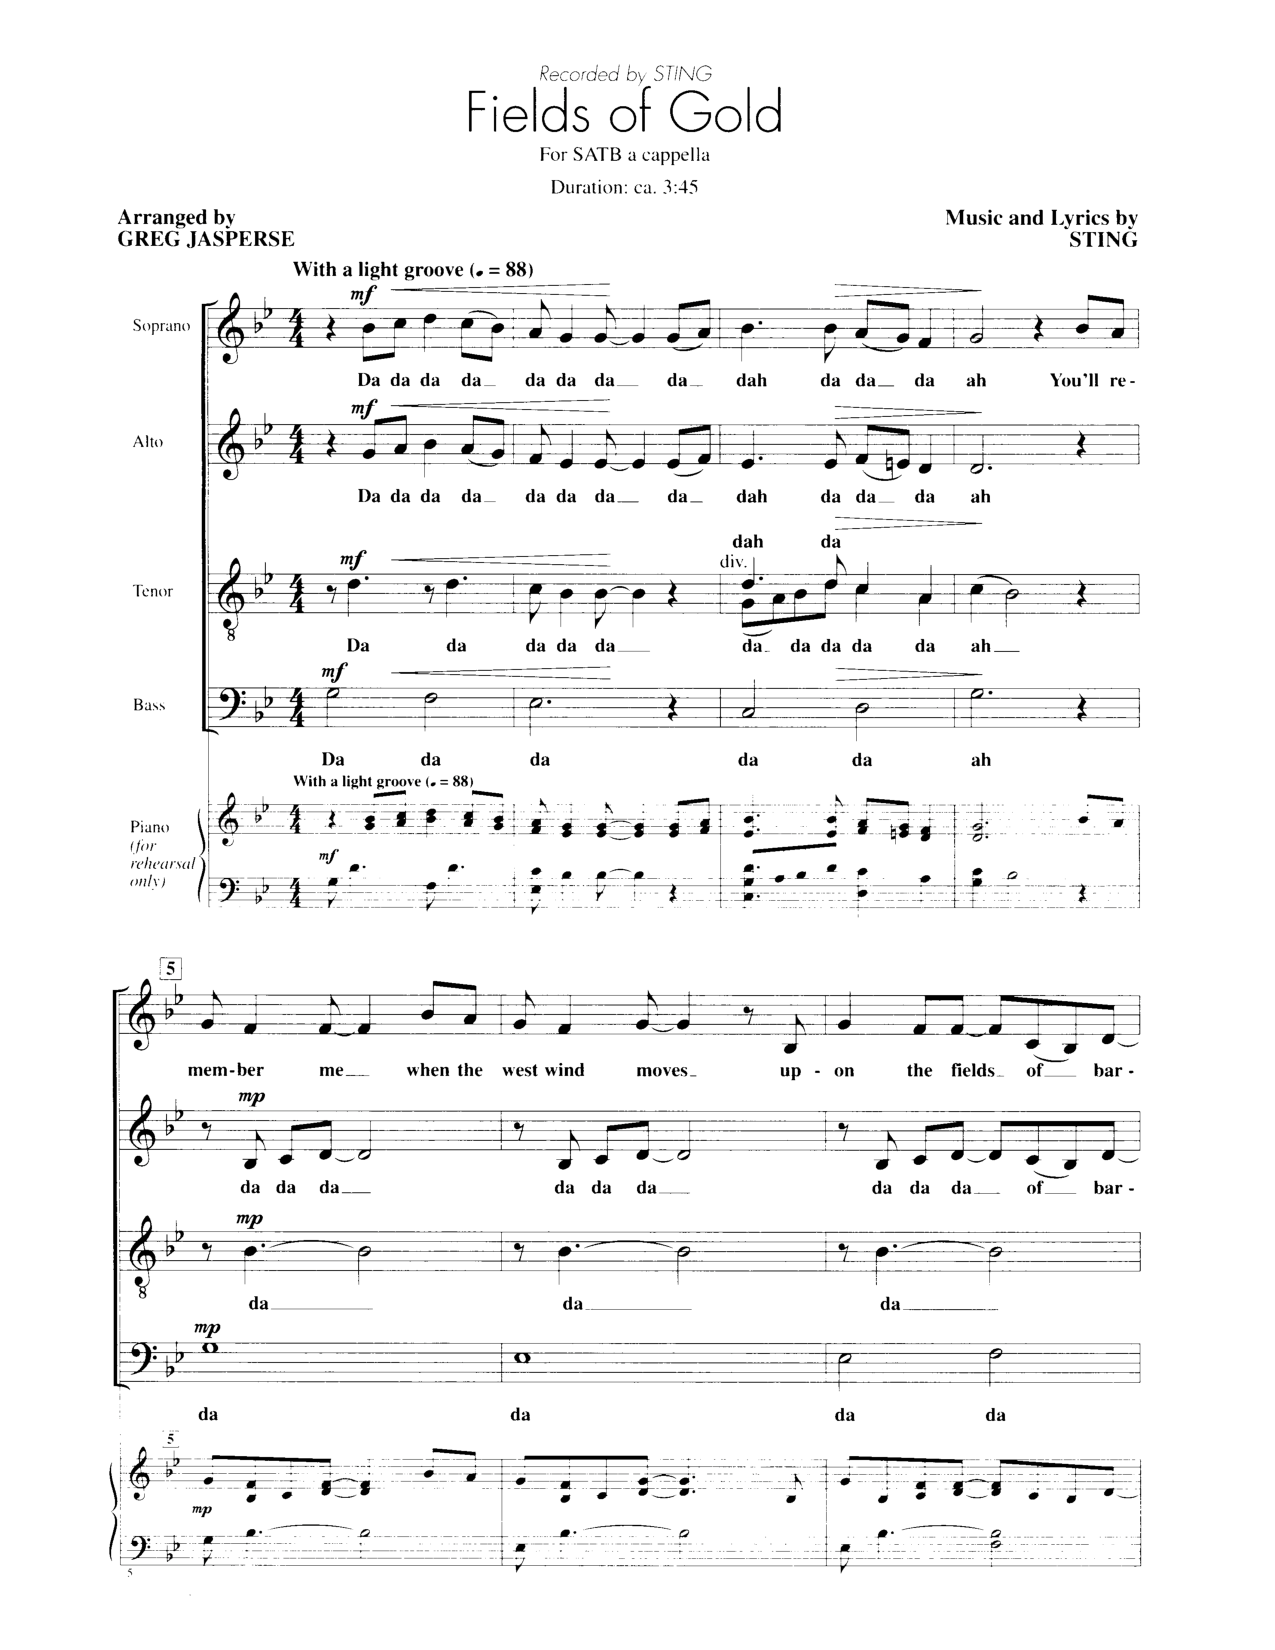
\includepdf[pages=-]{resources/arrangements/Fields Of Gold.pdf}
\label{appendix:Fields Of Gold} 


\end{document}
